\section{Zielsetzung}
\label{sec:Ziel}
In diesem Versuch werden die Zerfallskurven und Halbwertszeiten zweier radioaktiver Stoffe experimentell ermittelt. Um dies für kleine Halbwertszeiten durchführen zu können,
wird die Aktivierung mit Neutronen von stabilen Kernen angewendet.

\section{Theorie}
\label{sec:Theorie}
Besonders Atome großer Ordnungszahl brauchen eine größere Anzahl an Neutronen, um in  einem energetisch stabilen Zustand zu sein. Dabei liegt die Anzahl der Neutronen meist 
zwischen $\qty{20}{\percent}$ und $\qty{50}{\percent}$ über jener der Protonen, die durch die Ordnungszahl $Z$ des Atoms beschrieben wird.
Atomkerne, die ein ungünstiges Verhältnis von Neutronen und Protonen vorweisen, zerfallen durch Kernreaktionen bis sie schließlich in einen stabilen Endzustand gelangen.
Dieser Zerfallsprozess wird im folgenden Kapitel erläutert.

\subsection{Zerfall instabiler Isotope und Bestimmung der Halbwertszeit}
\label{subsec:Zerfall}
Der Zerfall von Atomkernen folgt einem exponentiellen Gesetz. Er kann mithilfe der Zerfallskonstante $\lambda$ des jeweiligen Isotopes über den Zusammenhang
\begin{equation}
    \label{eqn:Zerfallsgesetz}
    N(t)= N_0 \symup{e}^{\lambda t}
\end{equation}
beschrieben werden, wobei $N$ die Anzahl der Kerne zum Zeitpunkt $t$ angibt. $N_0$ ist demnach die Anzahl der vorhandenen Kerne zum Zeitpunkt $t=0$. 
Die Zeit, nach welcher genau die Hälfte der zuvor vorhandenen Kerne zerfallen ist, ist ebenfalls eine Konstante des Isotopes. Sie wird \textit{Halbwertszeit} $T$
genannt und kann über $N(T) = \sfrac{N_0}{2}$ zu 
\begin{equation}
    \label{eqn:Halbwertszeit}
    T = \frac{\symup{ln}(2)}{\lambda}
\end{equation}
bestimmt werden.
Da die Anzahl der vorhandenen Kerne nicht einfach festgestellt werden kann, wird meistens die Zahl der pro Zeitintervall $\symup{\Delta}t$ zerfallenen Kerne mit einem 
Geiger-Müller-Zählrohr gemessen. Die gemessene Größe lässt sich mit \autoref{eqn:Zerfallsgesetz} zu
\begin{equation}
    \label{eqn:N_dt}
    N_{\symup{\Delta}t}(t) = N(t)-N(t+ \symup{\Delta}t) = N_0 \left(1- \symup{e}^{-\lambda \symup{\Delta}t}\right) \cdot \symup{e}^{-\lambda t}
\end{equation}
bestimmen, was ebenfalls eine Proportionalität zum Exponentiallterm $\symup{e}^{-\lambda t}$ beinhaltet.
Durch diese Begebenheit lässt sich $\lambda$ durch Anwenden des Logarithmus auf beiden Seiten der Gleichung mittels linearer Ausgleichsrechnung ermitteln.

Der genaue Zerfallsprozess variiert je nach Isotop und kann über eine Zerfallsgleichung beschrieben werden. Im Falle der in diesem Versuch untersuchten Vanadium- ($\ce{^{52}_{23}V}$)
und Rhodium- ($\ce{^{104}_{45}Rh}$) Isotope folgen die Zerfälle den Gleichungen aus \autoref{fig:Zerfall_1}.

\begin{figure}
    \centering
    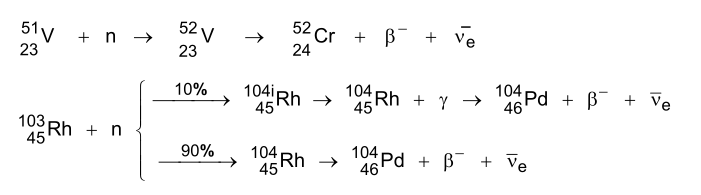
\includegraphics[width = .7\textwidth]{content/Zerfall_1.png}
    \caption{Zerfallsgleichungen von Vanadium und Rhodium \cite{v702}. Bei Rhodium können zwei unterschiedliche Zerfallsprozesse festgestellt werden.}
    \label{fig:Zerfall_1}
\end{figure}

\subsection{Aktivierung mit Neutronen}
\label{subsec:Aktivierung}
Wie bereits in der Einleitung erwähnt wurde, werden in diesem Versuch vergleichsweise geringe Halbwertszeiten im Bereich von Sekunden bis Stunden ermittelt. Da bei solchen 
Halbwertszeiten bereits nach geringer Zeit ein Großteil der instabilen Kerne zerfällt, müssen die Proben unmittelbar vor dem Durchführen des Versuches hergestellt werden.
Dies wird mithilfe der Aktivierung mit Neutronen erreicht.
Dabei werden (langsame) Neutronen auf einen stabilen Kern geschossen. Dringt ein Neutron in einen Kern ein, ensteht ein angeregeter Zwischenkern, der auch \textit{Compoundkern}
genannt wird. Durch die kinetische Energie und die Bindungsenergie des zugefügten Neutrons gehen die Nukleonen des Kerns in höhere Energiezustände über. Dies wird als 
\textit{Aufheizung} des Zwischenkerns bezeichnet. Durch Emission eines $\gamma$-Quants fällt der Kern nach kurzer Zeit (etwa $\qty{10e-16}{\second}$) wieder in den Grundzustand 
zurück. Da nun ein Neutron mehr vorhanden ist, ist der neue Kern meist instabil. Unter Emission eines Elektrons ($\beta$-Strahlung) kann er sich (eventuell über mehrere Prozesse)
in einen stabilen Kern umwandeln. Diese Kernreaktionen werden für einen Allgemienen Kern A mit Ordnungszahl $z$ und Massenzahl $m$ durch die Gleichungen aus 
\autoref{fig:Zerfall_2} beschrieben.

\begin{figure}
    \centering
    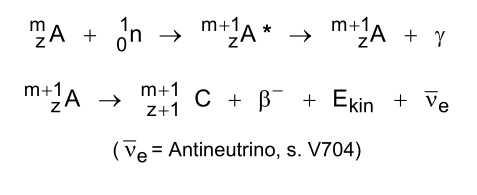
\includegraphics[width = .5\textwidth]{content/Zerfall_2.png}
    \caption{Zerfallsreaktionen bei der Neutronen Aktivierung \cite{v702}.}
    \label{fig:Zerfall_2}
\end{figure}

Neutronen sind als freie Teilchen instabil, weshalb sie durch andere Kernreaktionen erzeugt werden müssen. Dazu werden Beryllium-Kerne mit $\alpha$-Teilchen beschossen.
In diesem Versuch wird als Quelle der $\alpha$-Teilchen ein Radium-226 Strahler verwendet. 
Die Beryllium-Kerne fangen ein $\alpha$-Teilchen ein und reagieren unter Freisetzung eines Neutrons zu Kohlenstoff, was in \autoref{fig:Zerfall_3} dargestellt ist.

\begin{figure}
    \centering
    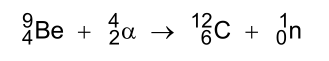
\includegraphics[width = .3\textwidth]{content/Zerfall_3.png}
    \caption{Kernreaktion eines Beryllium-Kerns mit einem $\alpha$-Teilchen \cite{v702}.}
    \label{fig:Zerfall_3}
\end{figure}

Da der Wirkungsquerschnitt $\sigma$, der die Wahrscheinlichkeit des Einfangs eines Neutrons beschreibt, reziprok proportional zur Geschwindigkeit $v$ der Neutronen ist, 
müssen die Neutronen zuerst abgebremst werden, bevor eine erfolgreiche Interaktion wahrscheinlich wird. Durch elastische Stöße mit anderen Teilchen kann diese Abbremsung
erreicht werden. Da dies für möglichst ähnliche Stoßmassen zur effektivsten Energieabgabe führt, wird ein Material mit leichten Atomkernen verwendet. In diesem Versuch wird
dazu Paraffin genutzt. Eine schematische Abbildung des Aufbaus der in diesem Versuch verwendeten Apparatur ist in \autoref{fig:Bottich} dargestellt.

\begin{figure}
    \centering
    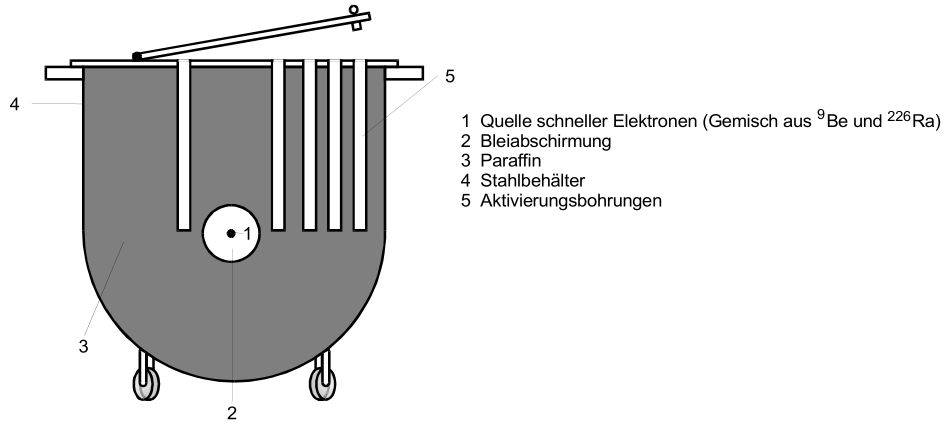
\includegraphics[width = .9\textwidth]{content/Bottich.png}
    \caption{Aufbau der verwendeten Neutronenquelle \cite{v702}.}
    \label{fig:Bottich}
\end{figure}

Nachdem die Neutronen einen Großteil ihrer Energie durch elastische Stöße abgegeben haben liegt ihre Energie bei ca. $\qty{0.025}{\electronvolt}$, was der Umgebungstemperatur 
entspricht. Die Neutronen sind dann etwa $\qty{2.2}{\kilo\metre\per\second}$ schnell und werden als \textit{thermische Neutronen} bezeichnet. 
